\subsection{\texorpdfstring{Lower Bound of $\Theta(C_{5})$}{Lower Bound of Theta(C5)}}

\begin{frame}
      \frametitle{Lower Bound of $\Theta(C_{5})$}

      \begin{figure}[h!]
            \tikzstyle{vertex}=[circle,fill=black!25,minimum size=20pt,inner sep=0pt]
            \tikzstyle{edge} = [draw,thick,-]
            \tikzstyle{weight} = [font=\small]
            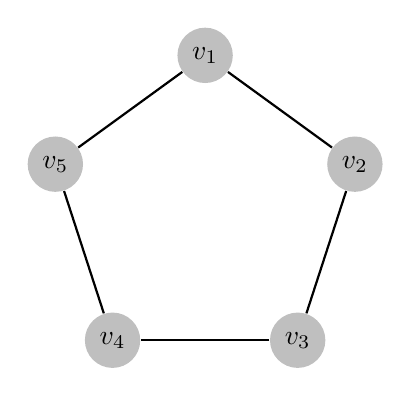
\begin{tikzpicture}[scale=1, auto,swap]
                  % Draw a 7,11 network
                  % First we draw the vertices
                  \foreach \pos/\name/\la in {{(0,2)/a/$v_{1}$},
                  {(1.902113032590307,0.6180339887498949)/b/$v_{2}$},
                  {(1.1755705045849465,-1.6180339887498947)/c/$v_{3}$},
                  {(-1.175570504584946,-1.618033988749895)/d/$v_{4}$},
                  {(-1.9021130325903073,0.6180339887498945)/e/$v_{5}$}}
                        \node[vertex] (\name) at \pos {\la};
                  % Connect vertices with edges and draw weights
                  \foreach \source/ \dest in {a/b,b/c,c/d,d/e,e/a}
                  \path[edge] (\source) -- node[weight]{} (\dest);
            \end{tikzpicture}
            \label{fig:Pentagon}
            \caption{$C_{5}$}
      \end{figure}

      The $ \alpha(C_{5}) $ is clearly equal to 2.

      \pause

      We want to show that $ \alpha((C_{5})^2) \ge 5 $.

      Thus $ \Theta(C_{5}) \ge \sqrt{\alpha((C_{5})^2)} \ge \sqrt{5} $
      
\end{frame}

\begin{frame}
      \frametitle{Lower Bound of $\Theta(C_{5})$}

      \begin{figure}[h!]
            \tikzstyle{vertexin}=[circle,fill=red!25,minimum size=20pt,inner sep=0pt]
            \tikzstyle{vertexout}=[circle,fill=green!25,minimum size=20pt,inner sep=0pt]
            \tikzstyle{edge} = [draw,thick,-]
            \tikzstyle{weight} = [font=\small]
            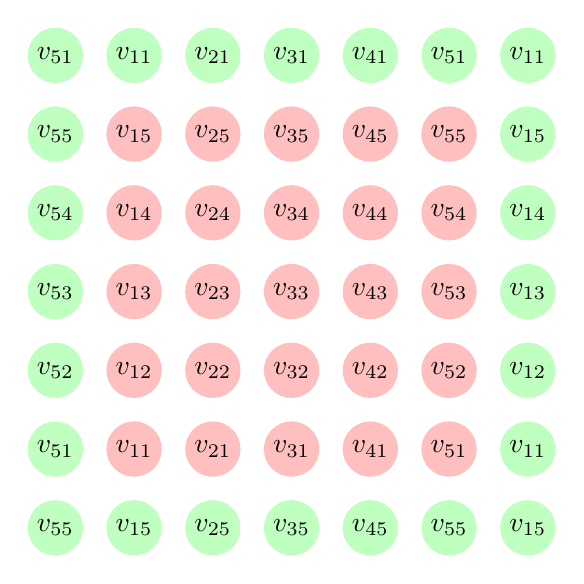
\begin{tikzpicture}[scale=1, auto,swap]
                  \foreach \i in {1,2,3,4,5}
                        \foreach \j in {1,2,3,4,5}
                              \node[vertexin] (v_{\i\j}) at (\i,\j) {$v_{\i\j}$};
                  
                  \node[vertexout] (v_{00}) at (0,0) {$v_{55}$};
                  \node[vertexout] (v_{01}) at (0,1) {$v_{51}$};
                  \node[vertexout] (v_{02}) at (0,2) {$v_{52}$};
                  \node[vertexout] (v_{03}) at (0,3) {$v_{53}$};
                  \node[vertexout] (v_{04}) at (0,4) {$v_{54}$};
                  \node[vertexout] (v_{05}) at (0,5) {$v_{55}$};

                  \node[vertexout] (v_{06}) at (0,6) {$v_{51}$};
                  \node[vertexout] (v_{16}) at (1,6) {$v_{11}$};
                  \node[vertexout] (v_{26}) at (2,6) {$v_{21}$};
                  \node[vertexout] (v_{36}) at (3,6) {$v_{31}$};
                  \node[vertexout] (v_{46}) at (4,6) {$v_{41}$};
                  \node[vertexout] (v_{56}) at (5,6) {$v_{51}$};

                  \node[vertexout] (v_{66}) at (6,6) {$v_{11}$};
                  \node[vertexout] (v_{65}) at (6,5) {$v_{15}$};
                  \node[vertexout] (v_{64}) at (6,4) {$v_{14}$};
                  \node[vertexout] (v_{63}) at (6,3) {$v_{13}$};
                  \node[vertexout] (v_{62}) at (6,2) {$v_{12}$};
                  \node[vertexout] (v_{61}) at (6,1) {$v_{11}$};

                  \node[vertexout] (v_{60}) at (6,0) {$v_{15}$};
                  \node[vertexout] (v_{50}) at (5,0) {$v_{55}$};
                  \node[vertexout] (v_{40}) at (4,0) {$v_{45}$};
                  \node[vertexout] (v_{30}) at (3,0) {$v_{35}$};
                  \node[vertexout] (v_{20}) at (2,0) {$v_{25}$};
                  \node[vertexout] (v_{10}) at (1,0) {$v_{15}$};
            \end{tikzpicture}
            \label{fig:Pentagon2}
            \caption{$(C_{5})^{2}$}
      \end{figure}

\end{frame}

\begin{frame}
      \frametitle{Lower Bound of $\Theta(C_{5})$}

      It is messy to draw edges in the graph of $(C_{5})^{2}$. So we use the following graph to give some idea of $(C_{5})^{2}$. But it is clear that every point is adjacent to the 8 points around it.

      Point $v_{ij}$ represent the vertex $(v_{i},v_{j})$ in $(C_{5})^{2}$.

      The green points are the same with the corresponding red points, we use it just for the convenience of visualization.

      \pause

      We will choose five points $v_{11}$, $v_{23}$, $v_{35}$, $v_{42}$, $v_{54}$, and show that they are mutually not adjacent.

\end{frame}

\begin{frame}
      \frametitle{Lower Bound of $\Theta(C_{5})$}

      \begin{figure}[h!]
            \tikzstyle{vertexin}=[circle,fill=red!25,minimum size=20pt,inner sep=0pt]
            \tikzstyle{vertexout}=[circle,fill=green!25,minimum size=20pt,inner sep=0pt]
            \tikzstyle{vertexs}=[circle,fill=blue!25,minimum size=20pt,inner sep=0pt]
            \tikzstyle{edge} = [draw,thick,-]
            \tikzstyle{weight} = [font=\small]
            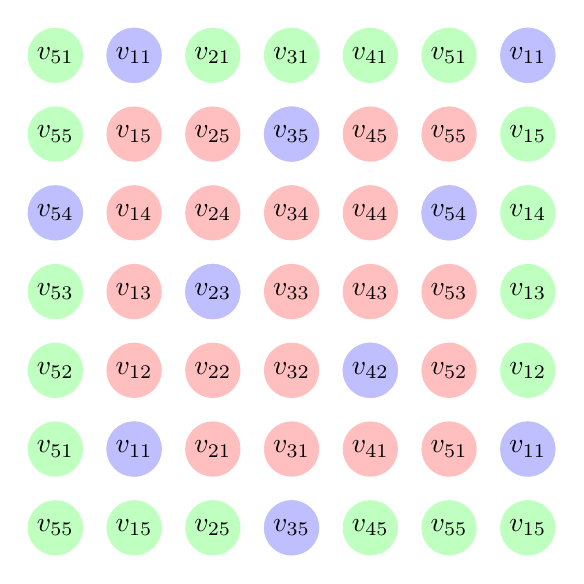
\begin{tikzpicture}[scale=1, auto,swap]
                  \foreach \i in {1,2,3,4,5}
                        \foreach \j in {1,2,3,4,5}
                              \node[vertexin] (v_{\i\j}) at (\i,\j) {$v_{\i\j}$};
                  
                  \node[vertexout] (v_{00}) at (0,0) {$v_{55}$};
                  \node[vertexout] (v_{01}) at (0,1) {$v_{51}$};
                  \node[vertexout] (v_{02}) at (0,2) {$v_{52}$};
                  \node[vertexout] (v_{03}) at (0,3) {$v_{53}$};
                  \node[vertexout] (v_{04}) at (0,4) {$v_{54}$};
                  \node[vertexout] (v_{05}) at (0,5) {$v_{55}$};

                  \node[vertexout] (v_{06}) at (0,6) {$v_{51}$};
                  \node[vertexout] (v_{16}) at (1,6) {$v_{11}$};
                  \node[vertexout] (v_{26}) at (2,6) {$v_{21}$};
                  \node[vertexout] (v_{36}) at (3,6) {$v_{31}$};
                  \node[vertexout] (v_{46}) at (4,6) {$v_{41}$};
                  \node[vertexout] (v_{56}) at (5,6) {$v_{51}$};

                  \node[vertexout] (v_{66}) at (6,6) {$v_{11}$};
                  \node[vertexout] (v_{65}) at (6,5) {$v_{15}$};
                  \node[vertexout] (v_{64}) at (6,4) {$v_{14}$};
                  \node[vertexout] (v_{63}) at (6,3) {$v_{13}$};
                  \node[vertexout] (v_{62}) at (6,2) {$v_{12}$};
                  \node[vertexout] (v_{61}) at (6,1) {$v_{11}$};

                  \node[vertexout] (v_{60}) at (6,0) {$v_{15}$};
                  \node[vertexout] (v_{50}) at (5,0) {$v_{55}$};
                  \node[vertexout] (v_{40}) at (4,0) {$v_{45}$};
                  \node[vertexout] (v_{30}) at (3,0) {$v_{35}$};
                  \node[vertexout] (v_{20}) at (2,0) {$v_{25}$};
                  \node[vertexout] (v_{10}) at (1,0) {$v_{15}$};

                  \node[vertexs] (v_{11}) at (1,1) {$v_{11}$};
                  \node[vertexs] (v_{66}) at (6,6) {$v_{11}$};
                  \node[vertexs] (v_{16}) at (1,6) {$v_{11}$};
                  \node[vertexs] (v_{61}) at (6,1) {$v_{11}$};

                  \node[vertexs] (v_{23}) at (2,3) {$v_{23}$};

                  \node[vertexs] (v_{35}) at (3,5) {$v_{35}$};
                  \node[vertexs] (v_{30}) at (3,0) {$v_{35}$};

                  \node[vertexs] (v_{42}) at (4,2) {$v_{42}$};

                  \node[vertexs] (v_{54}) at (5,4) {$v_{54}$};
                  \node[vertexs] (v_{04}) at (0,4) {$v_{54}$};

            \end{tikzpicture}
            \label{fig:Pentagon3}
            \caption{$(C_{5})^{2}$}
      \end{figure}

\end{frame}